\documentclass[pdf]
{beamer}
\usepackage[spanish]{babel}
\usepackage{graphicx}
\usetheme{Darmstadt}

\title{Leyes de Newton}
\subtitle{Laboratorio 03: Newton! Otra vez! D:}
\author{Fernando García \and Felipe Colli }
\date{31 de marzo de 2026}

\titlegraphic{
\includegraphics[height=1.5cm]{logo_fcfm.png}}

\begin{document}

\begin{frame}
	\titlepage
\end{frame}

\begin{frame}{Biografia de Isaac Newton (1642 - 1727)}
	\begin{columns}
		\column{0.6\textwidth}
		\textbf{Breve Biografía:}
		\begin{itemize}
			\item Fue un físico, teólogo, inventor, alquimista y matemático inglés.
			\item Es autor de los libros llamados Principia mathematica, donde describió la ley de la gravitación universal.
			\item Estableció las bases de la mecánica clásica mediante las leyes que llevan su nombre.
			\item También aporto con sus trabajos sobre la naturaleza de la luz y el desarrollo del cálculo.
		\end{itemize}

		\column{0.4\textwidth}
		\centering
		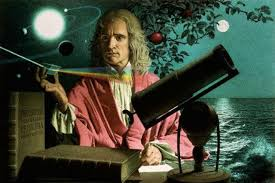
\includegraphics[width=0.8\textwidth]{newton.jpg} \\
		\footnotesize{Sir Isaac Newton}
	\end{columns}
\end{frame}

\begin{frame}{Primera Ley de Newton: Ley de la Inercia}
	\textbf{Descripción:} \\
	Todo cuerpo preserva su estado de reposo o movimiento rectilíneo uniforme a no ser que sea obligado a cambiar su estado por fuerzas afectadas sobre él \cite{valdivia_fisica_cap3}.

	\vspace{0.5cm}
	\textbf{Ecuación:}
	\[ \sum \vec{F} = 0 \iff \vec{v} = \text{constante} \quad (\text{o } \vec{v} = 0) \]

	\vspace{0.5cm}
	\textbf{Ejemplo en la vida cotidiana:}
	\begin{itemize}
		\item Cuando vas en la micro y frena de golpe, tu cuerpo tiende a seguir moviéndose hacia adelante debido a la inercia.
	\end{itemize}
\end{frame}

\begin{frame}{Segunda Ley de Newton: La fuerza es directamente proporcional a la aceleración}
	\begin{block}{Descripción}
		El cambio de movimiento es directamente proporcional a la fuerza motriz impresa y ocurre según la línea recta a lo largo de la cual aquella fuerza se imprime \cite{nasa_newton_laws}.
	\end{block}

	\begin{block}{Ecuación}
		\[ \vec{F} = m \cdot \vec{a} \]
		\centering \small{(La fuerza neta es igual a la masa por la aceleración)}
	\end{block}
	\begin{block}{Ejemplo en la vida cotidiana}
		Empujar un auto en pana. Si en vez de ser un auto es un camión pesado , necesitarás aplicar mucha más fuerza para lograr que se mueva que si estuvieras empujando un auto pequeño.
	\end{block}
\end{frame}
\begin{frame}{Tercera Ley de Newton: Acción y Reacción}
	\textbf{Definición:} \\
	Con toda acción ocurre siempre una reacción igual y contraria: es decir, las fuerzas mutuas de dos cuerpos siempre son de igual magnitud y dirigidas en sentido opuesto \cite{nasa_newton_laws, valdivia_fisica_cap3}.

	\vspace{0.5cm}
	\textbf{Ecuación que la modela:}
	\[ \vec{F}_{A \to B} = -\vec{F}_{B \to A} \]

	\vspace{0.5cm}
	\textbf{Ejemplo en la vida cotidiana:}
	\begin{itemize}
		\item Al nadar, empujas el agua hacia atrás con tus manos, y el agua te empuja hacia adelante con la misma magnitud de fuerza.
	\end{itemize}
\end{frame}
\begin{frame}{Bibliografía}
	\bibliographystyle{plain}
	\bibliography{bibliografia}
\end{frame}
\end{document}
